\documentclass{article}
\usepackage{graphicx} % Required for inserting images
\usepackage{amsmath}
\usepackage{tikz}
\usetikzlibrary{shapes.gates.logic.US, positioning}
\title{1.9}
\author{Mokshith Kumar Reddy }
\date{February 2025}

\begin{document}

\maketitle
\section{Binary Logic}
Binary logic deals with variables that take on two discrete values(most commonly 0 and 1) and with operations that assume logical meaning.\\[10pt]
The binary logic introduced in this is equivalent to an algebra called Boolean algebra.\\[10pt]
\textbf{Definition of Binary Logic}\\
Binary logic consists of binary variables and a set of logical operations. There are three basic logical operations: AND, OR, and NOT. Each operation produces a binary result.\\[10pt ]
For each combination of the values of x and y, there is a value of z specified by the
definition of the logical operation. Definitions of logical operations may be listed in a
compact form called truth tables.\\[10pt]
\textbf{AND:}\\[10pt]The logical operation AND is interpreted to mean that z = 1 if and only if x = 1 and y= 1; otherwise z = 0 (The result of the operation $x\cdot y$ is z).
\begin{itemize}
        \item Truth table:
        \begin{tabular}{|c|c|c|}
        \hline
        x & y & x $\cdot$ y \\
        \hline
        0 & 0 & 0 \\
        \hline
        0 & 1 & 0 \\
        \hline
        1 & 0 & 0 \\
        \hline
        1 & 1 & 1 \\
        \hline
        \end{tabular}
\end{itemize}
\textbf{OR:}\\[10pt] The output z = 1 if x = 1 or if y= 1 or if both x = 1
and y= 1. If both x = 0 and y= 0, then z = 0.This operation is represented by a plus sign.\\
\begin{itemize}
        \item Truth table:
        \begin{tabular}{|c|c|c|}
        \hline
        x & y & x + y \\
        \hline
        0 & 0 & 0 \\
        \hline
        0 & 1 & 1 \\
        \hline
        1 & 0 & 1 \\
        \hline
        1 & 1 & 1 \\
        \hline
        \end{tabular}
\end{itemize}
\textbf{NOT:}\\[10pt]
The NOT operation is also referred to as the complement operation, since it changes a 1 to 0 and a 0 to 1, that is, the result of complementing 1 is 0, and vice versa. This operation is represented by a prime (sometimes by an overbar).
\begin{itemize}
        \item Truth table:
        \begin{tabular}{|c|c|}
        \hline
        x & x' \\
        \hline
        0 & 1 \\
        \hline
        1 & 0 \\
        \hline
        \end{tabular}
\end{itemize}
*binary logic should not be confused with binary arithmetic.\\[10pt]
\textbf{Logic Gates}\\[10pt]
Logic Gates are electronic circuits that process input signals (voltages or currents) to produce binary outputs (0 or 1).
\begin{itemize}
    \item \textbf{Digital System:} Defines:
    \begin{itemize}
        \item Logic 0: $0 \, \text{V}$
        \item Logic 1: High Voltage $ \, \text{V}(3 \text{V})$
    \end{itemize}
\end{itemize}
Logic gates interpret binary input signals and produce corresponding binary. \\
The timing diagrams illustrate the idealized response of each gate to the
four input signal combinations. The horizontal axis of the timing diagram represents the time, and the vertical axis shows the signal as it changes between the two possible
voltage levels.\\
\begin{figure}[h]
\centering
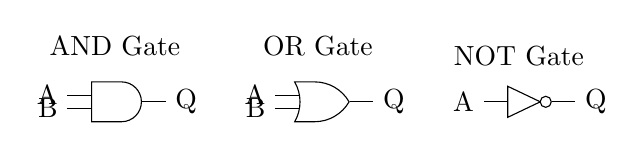
\begin{tikzpicture}[
    gate/.style={draw, thick, minimum width=12mm, minimum height=20mm},
    node distance=20mm
]

% AND Gate
\node[and gate US, draw] (and) {};
\draw (and.input 1) -- ++(-0.3,0) node[left] {A};
\draw (and.input 2) -- ++(-0.3,0) node[left] {B};
\draw (and.output) -- ++(0.3,0) node[right] {Q};

% OR Gate (positioned to the right of AND gate)
\node[or gate US, draw, right=of and] (or) {};
\draw (or.input 1) -- ++(-0.3,0) node[left] {A};
\draw (or.input 2) -- ++(-0.3,0) node[left] {B};
\draw (or.output) -- ++(0.3,0) node[right] {Q};

% NOT Gate (positioned to the right of OR gate)
\node[not gate US, draw, right=of or] (not) {};
\draw (not.input) -- ++(-0.3,0) node[left] {A};
\draw (not.output) -- ++(0.3,0) node[right] {Q};

% Labels
\node[above=2mm] at (and.north) {AND Gate};
\node[above=2mm] at (or.north) {OR Gate};
\node[above=2mm] at (not.north) {NOT Gate};

\end{tikzpicture}
\caption{Basic logic gates with standard symbols and labels.}
\label{fig:logic_gates}
\end{figure}

\textbf{Gates with Multiple Inputs}
\begin{itemize}
    \item \text{Three-input AND Gate:} Outputs $1$ if all inputs are $1$.
    \item \text{Four-input OR Gate:} Outputs $1$ if any input is $1$; outputs $0$ only if all inputs are $0$.
\end{itemize}
\end{document}
